\documentclass[book.tex]{subfiles}
\begin{document}
\section{Getting the Source Code}
The game engine source code was released on July 21st, 1995. It was uploaded on id software's ftp\footnote{File Transfer Protocol.} server.\\ 
\par
\begin{minipage}{\textwidth}
\lstinputlisting[]{code/ftp_url.txt}
\end{minipage}
\par
More than twenty two years later the archive is still there, at the exact same URL. A remarkable fact given the ever changing nature of the web.\\

\section{First Contact}
Once downloaded and decompressed, it turns out the archive \codeword{woldsrc.zip} contains an other self-extracting PKZIP archive. It was a convenience back in the day but it is not practical now. It is easy to deflate.\\
\par
\begin{minipage}{\textwidth}
\lstinputlisting{code/unzip.txt}
\end{minipage}

\par
\cw{cloc.py} is a tool which will look at every files in a folder and gather statistics about source code. It helps to get an idea of what to expect.\\
\par

\begin{minipage}{\textwidth}
\lstinputlisting[]{code/cloc.txt}
\end{minipage}

\par
 The code is 90\% in C with assembly for bottleneck optimizations and low level I/O such as video or audio\footnote{id Software would not switch to C++ until Doom 3 around 2000.}. Lines of code is not a meaningful metric against a single codebase but it excels when it comes to extracting proportions. Wolfenstein 3D with its 27,223 SLOC is very small compared to most software. \cw{curl} (a command-line tool to download url content) is 154,134 SLOC. Chrome (Google's web browser) is 1,700,000 SLOC. Linux kernel is 15,000,000 SLOC.\\
\par
\begin{figure}[H]
\centering
  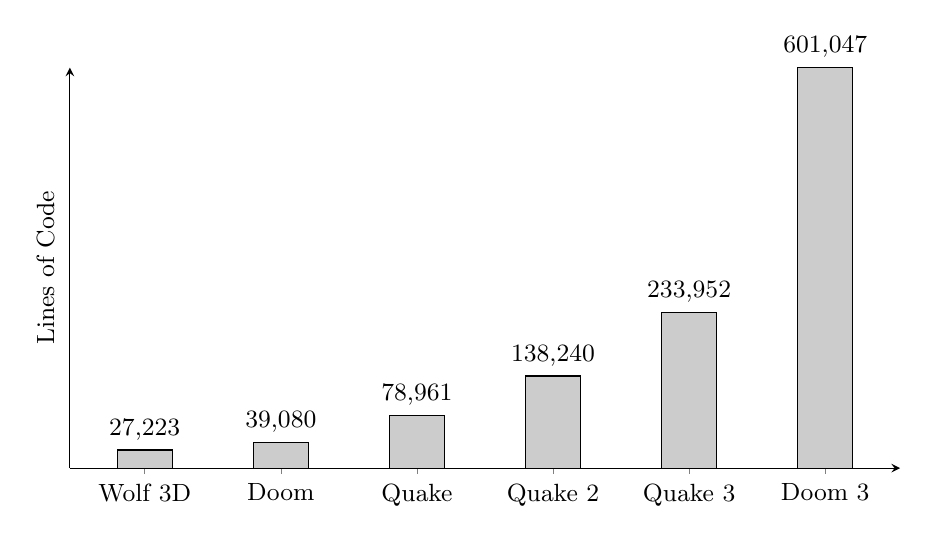
\begin{tikzpicture}[font=\small]
    \begin{axis}[
      width=\textwidth,
      height=0.55\textwidth,
      ybar=0.6\textwidth,
      bar width=20pt,
      ylabel={Lines of Code},
      ymin=0,
      ytick=\empty,
      xtick=data,
      axis x line=bottom,
      axis y line=left,
      enlarge x limits=0.11,
      symbolic x coords={Wolf 3D,Doom,Quake,Quake 2,Quake 3, Doom 3},
      xticklabel style={},
      yticklabel style={},
      nodes near coords={\pgfmathprintnumber[fixed,precision=0]\pgfplotspointmeta}
    ]
      \addplot[fill=black!20,draw=black] coordinates {
        (Wolf 3D,27223)
        (Doom,39080)
        (Quake,78961)
        (Quake 2, 138240)
        (Quake 3, 233952)
        (Doom 3, 601047)
      };
    \end{axis}
   \end{tikzpicture} 
   \caption{Line of codes from id Software game engines.}
 \end{figure}
 
\par

 \begin{fancyquotes}
   We didn't have spell checkers in our editors back then, and I always had poor spelling.  The word "collumn" appears in the source code dozens of times.  After I released the source code, one of the emails that stands out in memory read:
 \bigskip \\
It's "COLUMN", you dumb FUCK!\\
 \bigskip \\
\textbf{John Carmack - Programmer}
 \end{fancyquotes}
 
The archive contains more than just source code, it also features:
\begin{itemize}
\item \codeword{GOODSTUF.TXT:} Two emails from fans demonstrating the success of the game: An ex-POW and a Microsoft employee.
\item \codeword{SIGNON.OBJ:} The startup screen showing the system characteristic (RAM, EMS, XMS, Joystick, SoundCards) was linked in the binary. This weird design choice is explained later.
\item \codeword{GAMEPAL.OBJ:} Game palette. Hardcoded and linked in the executable for the same reason as \cw{SIGNON.OBJ}.
\item \codeword{README:} How to build. You can also find a complete tutorial on the author's article "Let's compile like its 1993" on \cw{fabiensanglard.net}.
\item Many files resulting from a previous compilation attempt.
\end{itemize}







\section{Big picture}
The game engine is divided in three blocks:
\begin{itemize}
\item The 2D menu engine which lets the user configure the game.
\item The 3D game renderer where the player spent more of her time.
\item The sound system which runs concurrently with either the 2D or 3D renderer. 
\end{itemize}
The three systems communicate via shared memory. The renderer writes music and sound request to the RAM (also making sure the assets are ready). These requests are read by the sound "loop". The sound system also write to the RAM for the renderers since it is in charge of the heartbeat of the whole engine. The renderers update the world according to the wall-time tracked by \cw{TimeCount} variable.
\par
\begin{figure}[H]
\centering
 \includegraphics[width=\textwidth]{imgs/drawings/three_systems.pdf}
 \end{figure}
 \par

 









\subsection{Unrolled loop}
With the big picture in mind, we can dive into the code and unroll the main loop starting in \cw{int main()}. The two renderers are regular loops but due to limitation explained later, the sound system is interrupt driven and therefore out of \cw{main}. Because of the Real Mode, C types don't mean what people would expect from a 32 bits architecture.
\begin{itemize}
\item \cw{int} and \cw{word} are 16 bits.
\item \cw{long} and \cw{dword} are 32 bits.
\end{itemize}
\par
Here is where the program starts.\\
\par
\begin{minipage}{\textwidth}
\lstinputlisting[language=C]{code/unrolled_loop_main.c}
\end{minipage}
\par

\par
In \cw{InitGame}, the engine starts up and bring up all the managers (those are described in details later).\\
\par
\begin{minipage}{\textwidth}
\lstinputlisting[language=C]{code/unrolled_loop_init.c}
\end{minipage}
\par
Then come the core loop where 2D renderer and 3D renderer are called forever.\\
\par
\begin{minipage}{\textwidth}
\lstinputlisting[language=C]{code/unrolled_loop_demoloop.c}
\end{minipage}
\par
\cw{PlayLoop} contains the 3D renderer. It is pretty standard with a get inputs, update world, render world approach.\\
\par
\begin{minipage}{\textwidth}
\lstinputlisting[language=C]{code/unrolled_loop_playloop.c}
\end{minipage}
\par
The sound system is started via the Sound Manager in \cw{SDL\_SetTimerSpeed}. There is a famous game development library called Simple DirectMedia Layer (SDL) but the prefix \cw{SDL\_} has nothing to do with it. It stands for SounD Low level. SDL did not even exist in 1991.\\
\par
The reason for interrupts is extensively explained in the Chapter "Audio and Heartbeat". In short, with an OS supporting neither process nor thread, it was the only way to have something execute concurrently with the rest of the engine.\\
\par
An ISR\footnote{Interrupt Service Routine} is installed in the Interrupt Vector Table to reponse to the interrupt. Note how the ISR can be called at frequencies of 140Hz, 700Hz or even 7000Hz depending on the needs of the sound system being driven.\\
\par
\begin{minipage}{\textwidth}
\lstinputlisting[language=C]{code/soundsystem_interrupt.c}
\end{minipage}
\par
















\section{Architecture}

The source code is structured in two layers. WL\_* files are high-level layers relying on low-level ID\_* sub-systems called Managers interacting with the hardware.\\
\par
 \par
\begin{figure}[H]
\centering
 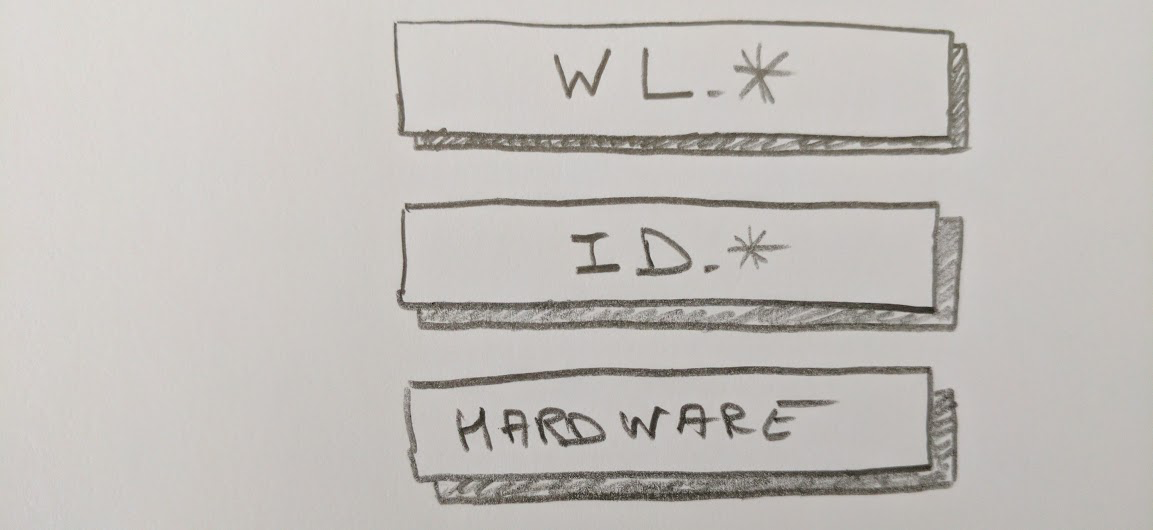
\includegraphics[width=\textwidth]{imgs/drawings/layers.png}
 \end{figure}
 \par
\par
There are seven managers in total:\\
\begin{itemize}
	\item Memory
	\item Page
	\item Video
	\item Cache
	\item Sound
	\item User
	\item Input
\end{itemize}
The WL\_ stuff was written specifically for Wolf3D while the ID\_ managers were reused from previous games (likely Catacomb 3D) and improved for the needs of the new engine.
\note{What does L stands for in WL ?}
\begin{figure}[H]
\centering
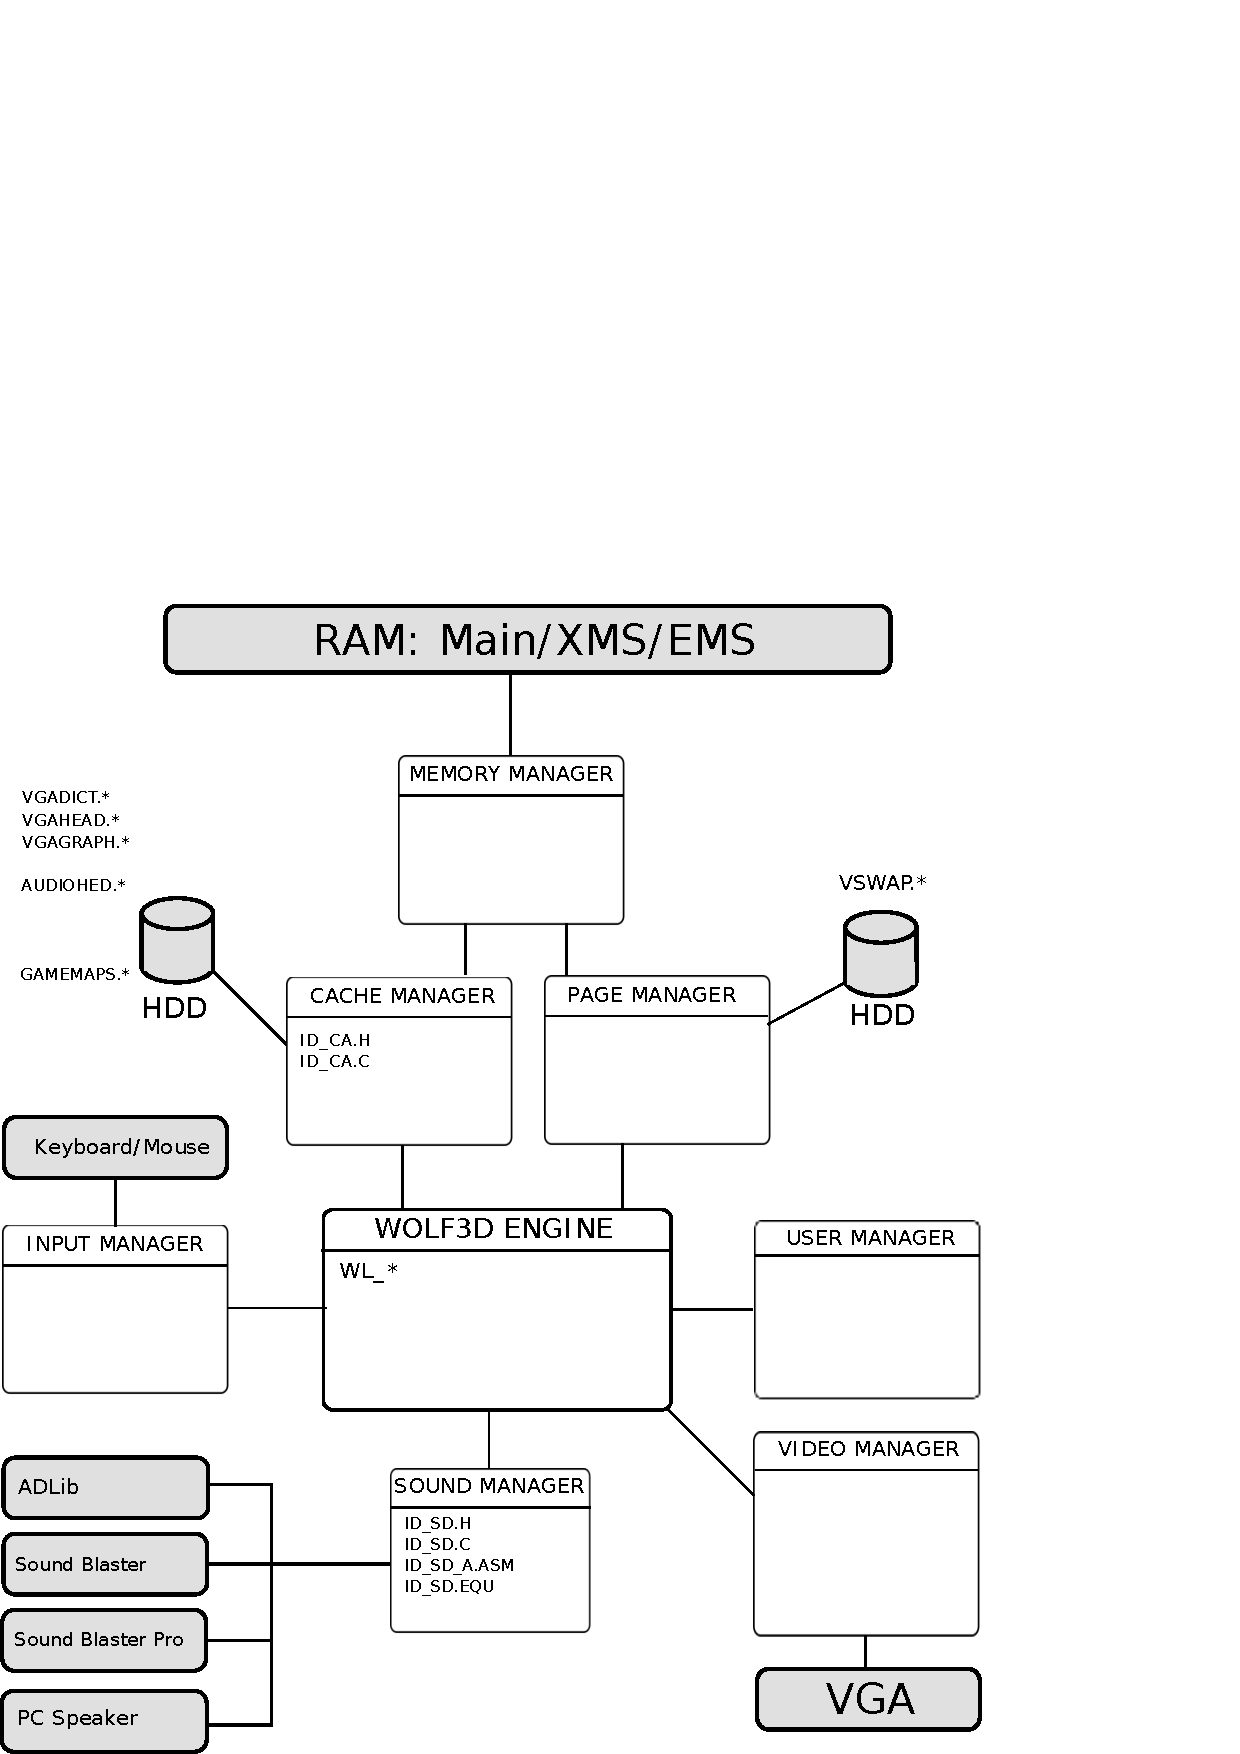
\includegraphics[width=\textwidth]{imgs/drawings/architecture.pdf}
\caption{Architecture with engine and sub-systems (in white) connected to I/O (in gray).}
\label{fig:architecture}
\end{figure}
Next to the hard drives (HDD) you can see the assets packed as described in the Team chapter.










\subsection{Memory Manager (MM)}
The engine does not rely on \cw{malloc} to manage conventionnal memory because it can lead to fragmented memory and no way to compact free space. It has its own memory manager made of a linked list of "block" keeping track of the RAM. A block points to a starting point in RAM and has a size.\\
 \par
\lstinputlisting[language=C]{code/mm_block.c}
 \par
A block can be marked with attributes:
\begin{itemize}
\item \cw{LOCKBIT} : This block of RAM cannot be moved during garbage collection.
\item \cw{PURGEBITS} : 0-3 level, 0= unpurgable, 1= purgable, 2= ???, 3= purge first.
\end{itemize}

The memory manager starts by allocating all available RAM via \cw{malloc}/\cw{farmalloc} and creates a \cw{LOCKED} block of size 1KiB at the end. The linked list uses two pointers: \cw{HEAD} and \cw{ROVER} which point on the second to last block.
 \par
\begin{figure}[H]
\centering
 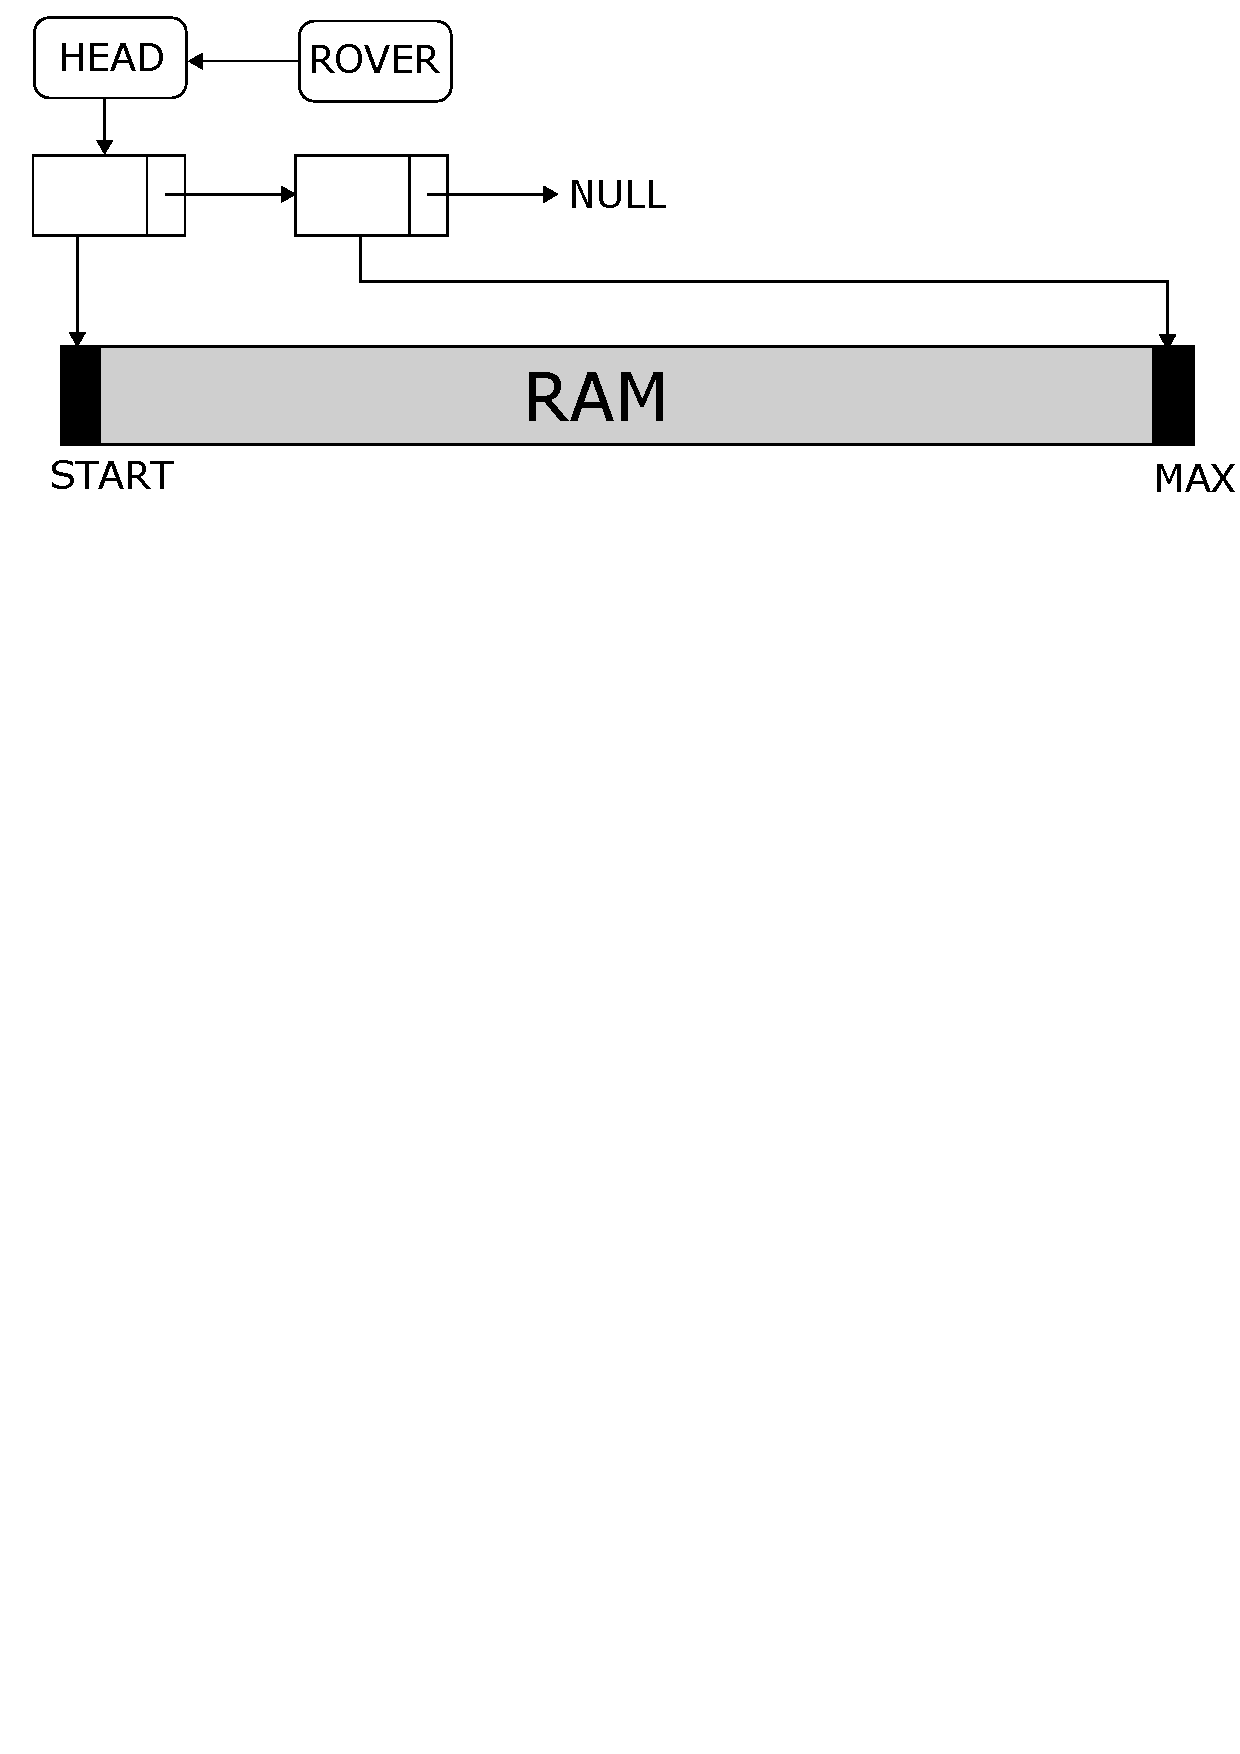
\includegraphics[width=\textwidth]{imgs/drawings/mm_start.pdf}
 \end{figure}
 \par
 The engine interacts with the Memory Manager by requesting RAM (\cw{MM\_GetPtr}) and freeing RAM (\cw{MM\_FreePtr}). To allocate memory, the manager searches for "holes" between blocks. It can take up to three passes of increasing complexity:
\begin{enumerate}
\item After rover.
\item After head.
\item Compacting and then after rover.
\end{enumerate}
\par
  The easier case is when there is enough space after the rover. A new node is simply added to the linked list and the rover moves forward. In the next drawing, three allocation requests succeeded: \cw{A}, \cw{B} and \cw{C}.\\
  \par
\begin{figure}[H]
\centering
 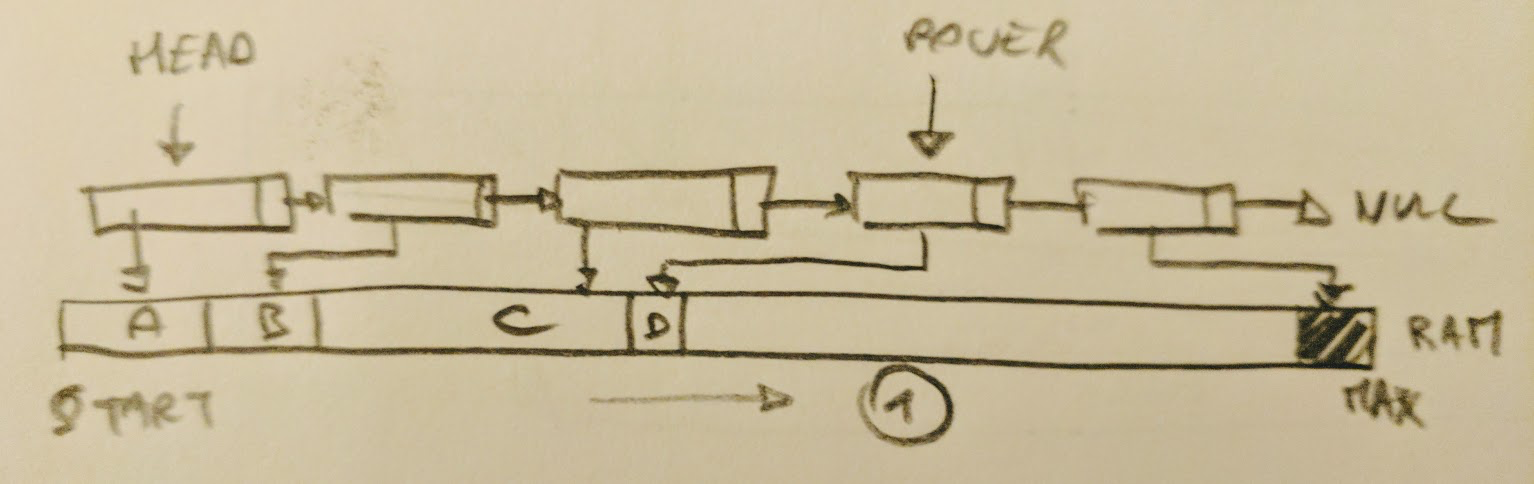
\includegraphics[width=\textwidth]{imgs/drawings/mm_after_rover.pdf}
 \caption{MM internal state after three pass 1 allocations.}
 \end{figure}
 \par
Eventually the free RAM will be exhausted and the first pass will fail.
  \par
\begin{figure}[H]
\centering
 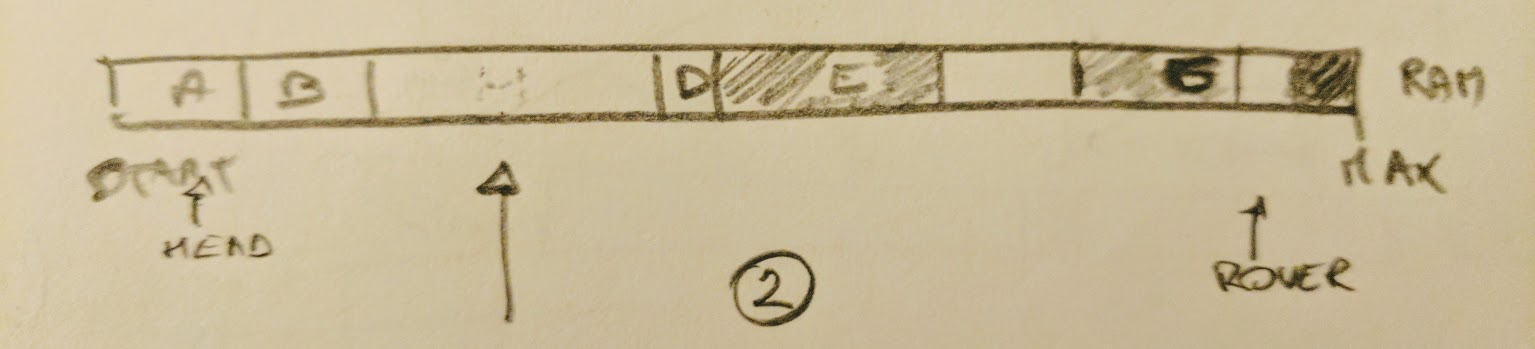
\includegraphics[width=\textwidth]{imgs/drawings/mm_before_rover.pdf}
 \caption{Pass 1 failure: Not enough RAM after the ROVER.}
 \end{figure}
 \par
 If the first pass fails, the second pass looks for a "hole" between the head and the rover. This pass is also allowed to purge unused block. If for example block B was marked as \cw{PURGEABLE}, it will be deleted and replaced with the new block E. At this point fragmentation starts to appear (like if \cw{malloc} was used).\\
 \begin{figure}[H]
\centering
 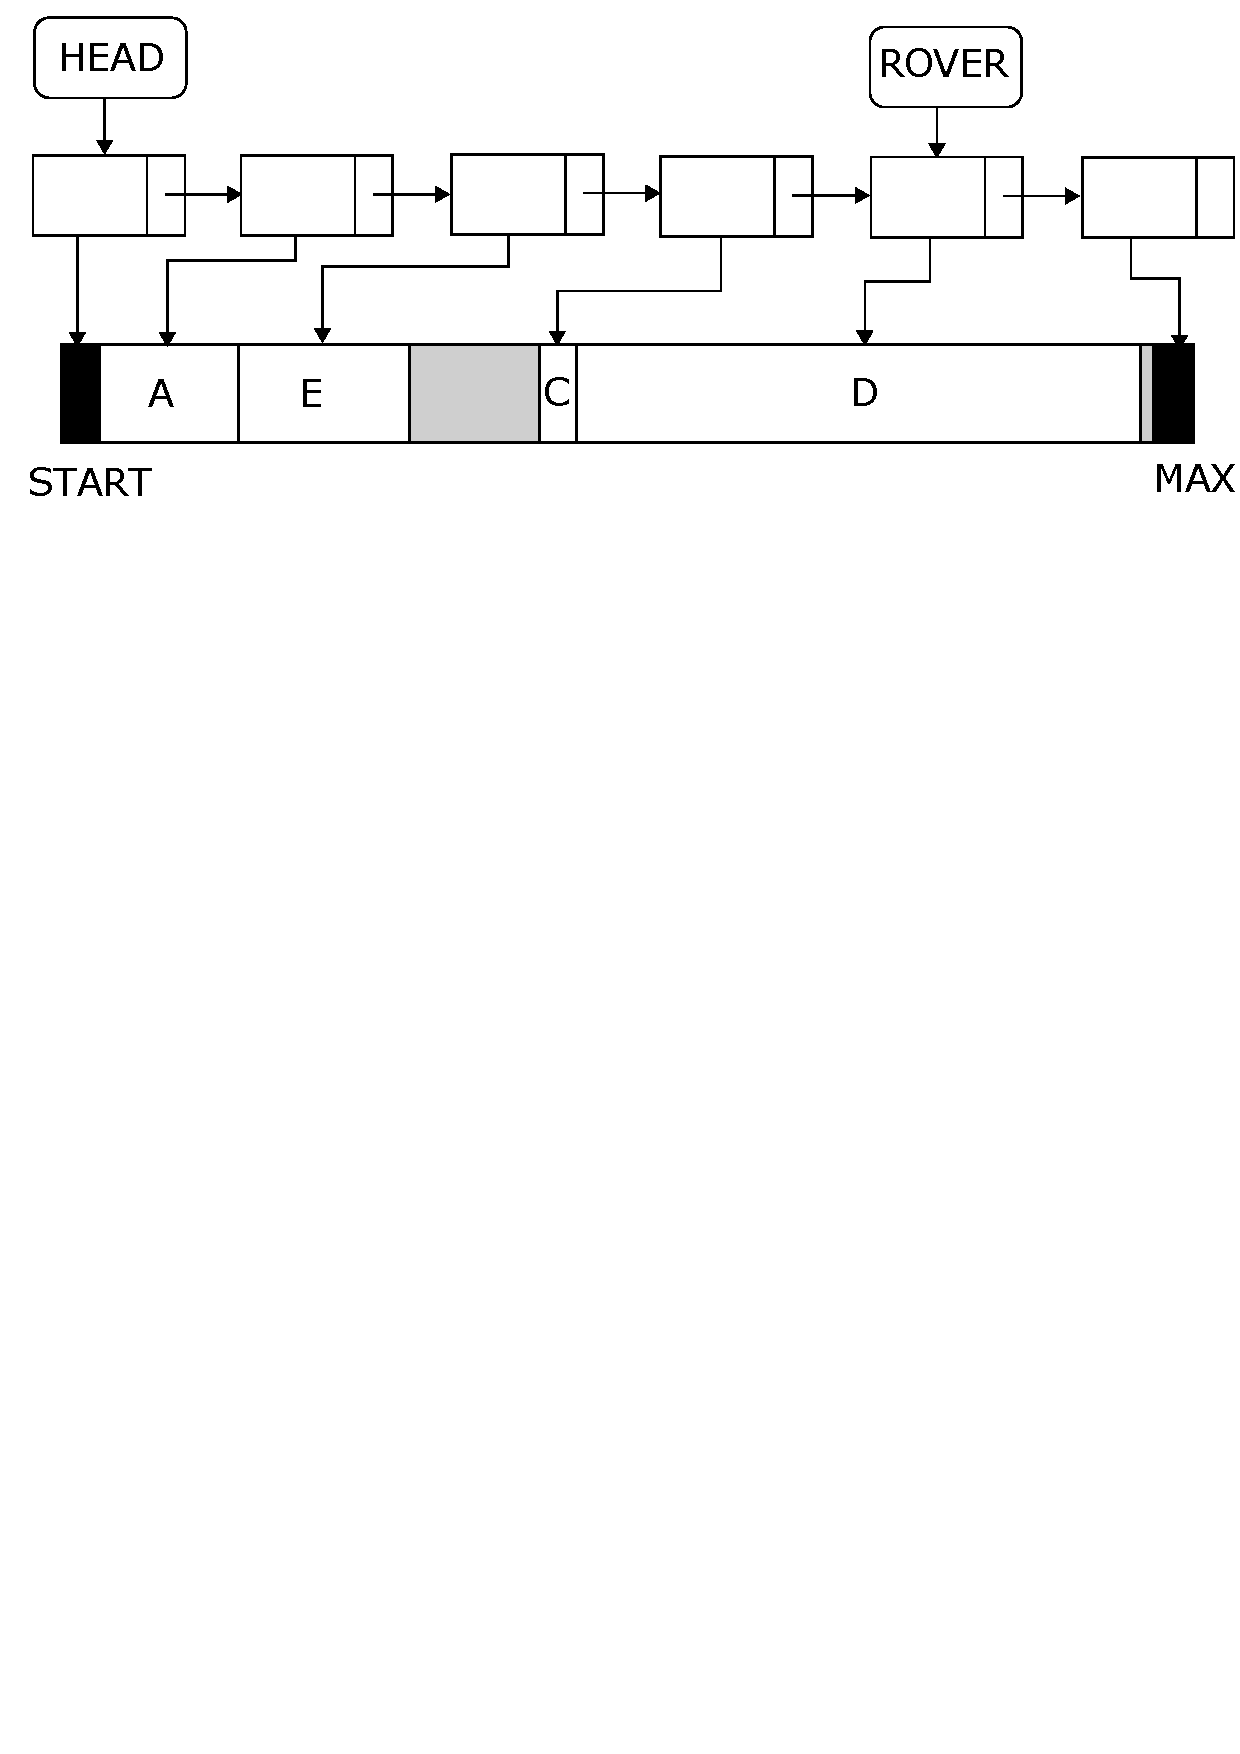
\includegraphics[width=\textwidth]{imgs/drawings/mm_after_head.pdf}
 \caption{\cw{B} was purged. \cw{E} was allocated in pass 2.}
 \end{figure}
 \par
 If the RAM reaches a point where the first and second pass failed, it means there is nowhere a continuous block of memory big enough to satisfy the request. The manager is going to iterate through the entire linked list and do two things: Delete blocks marked as purgeable and compact the RAM by moving blocks.
  \par
\begin{figure}[H]
\centering
 \includegraphics[width=\textwidth]{imgs/drawings/mm_compact.pdf}
  \caption{\cw{A} and \cw{E} were purged. \cw{C} and \cw{F} compacted. \cw{F} allocated in pass3.}
 \end{figure}
 \par
But if memory is moved around, how do previous allocation still point to what they had before the garbage collection phase? Notice that a \cw{mmblockstruct} has a \cw{useptr} pointer which point to the owner of a block: If it moves memory, it also updates the ower of the block.

   \par
\begin{figure}[H]
\centering
 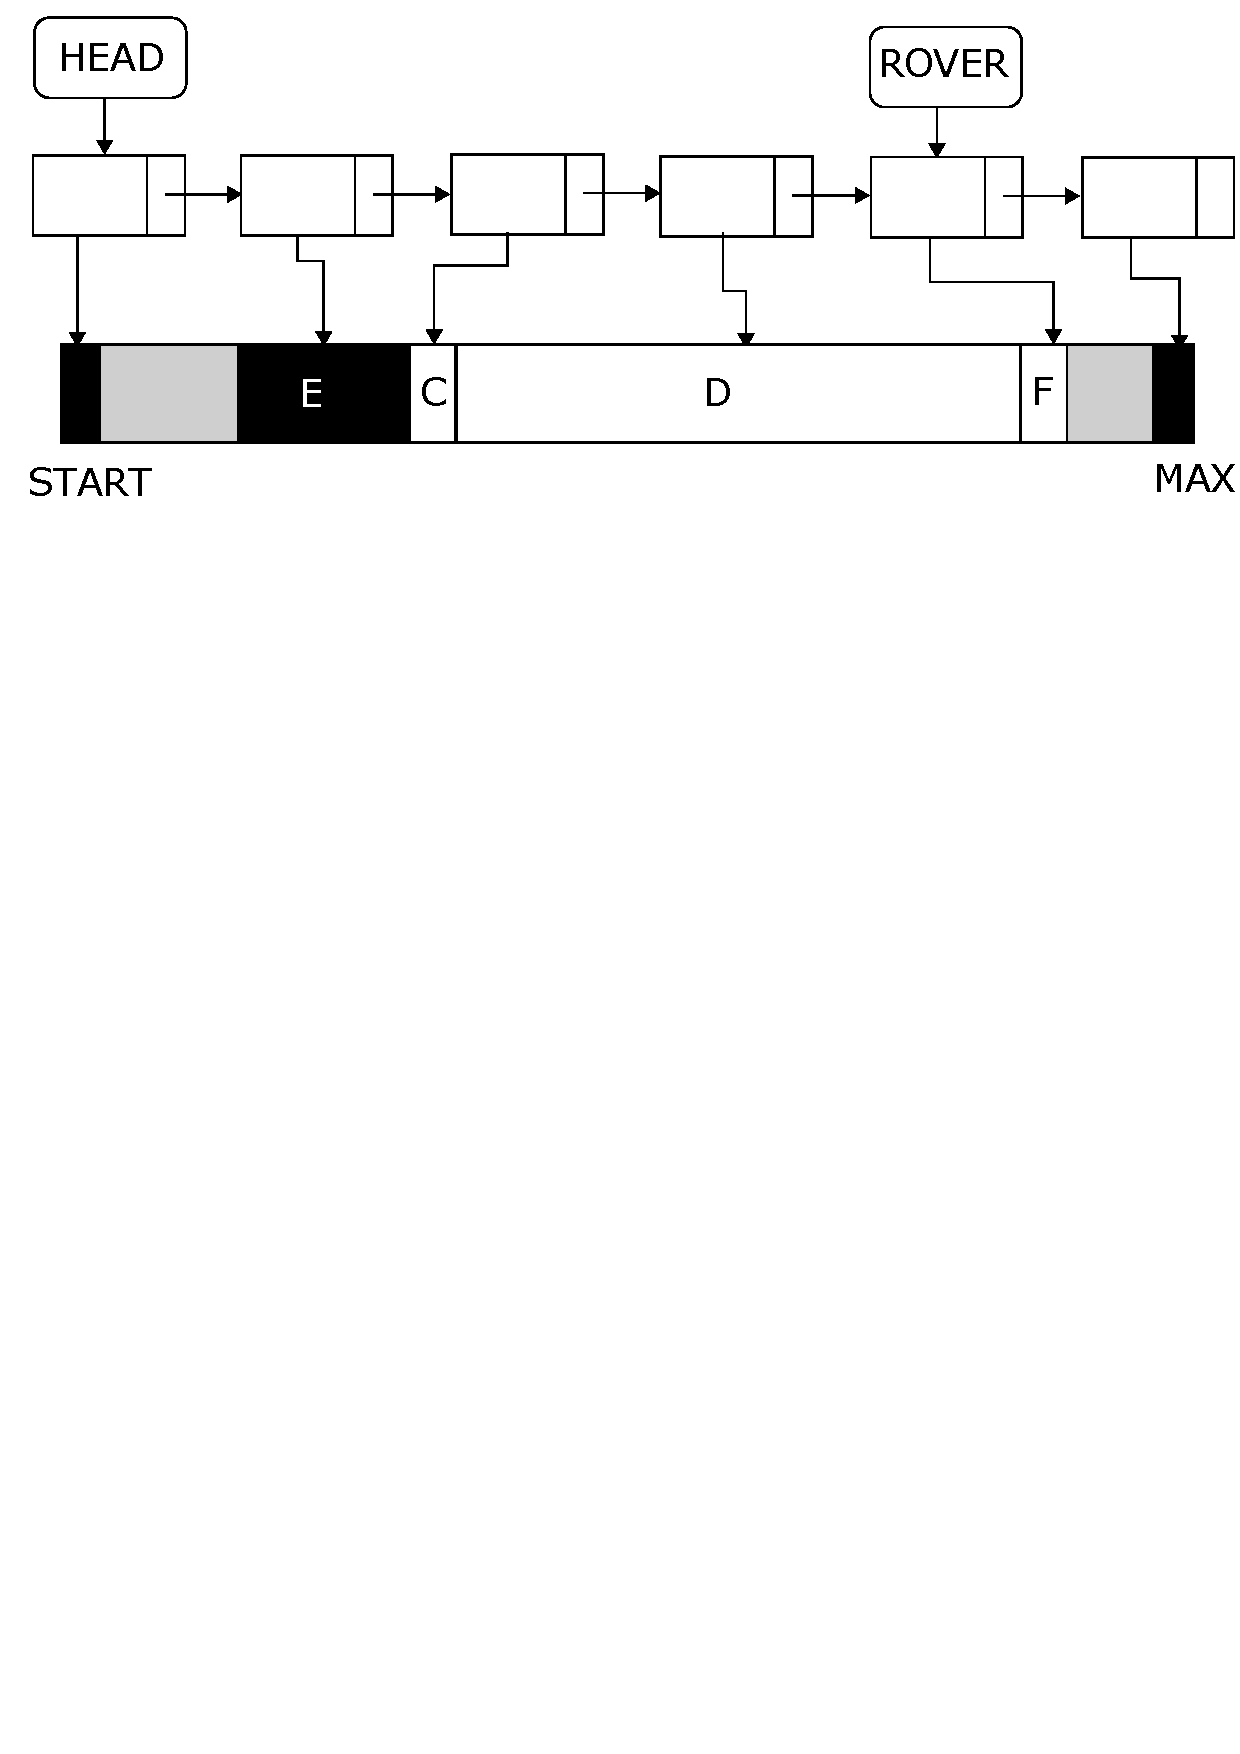
\includegraphics[width=\textwidth]{imgs/drawings/mm_bad_compact.pdf}
 \caption{\cw{E} is locked and cannot be compacted.}
 \end{figure}
 \par
 Because some blocks can be marked as \cw{LOCKED}, compacting can be disturbed. Upon encountering a locked lock, compacting stop and the next block will be moved immediately after the locked block, even is there was space available between the last block and the locked block. In the above drawing, C was moved after E, even though it could have been moved before. But avoiding this waste would have made the memory manager more complicated, that was an acceptable waste. Often in designing a component you have to be practical and establish a certain trade off between accuracy and complexity.












\subsection{Page Manager (PM)}
The Page Manager is dedicated to the 3D engine. Its task is to make sure assets such a wall texture, sprites and sound effect stored on HDD are available in RAM for the CPU to use. Jason Blochowiak seems to have been the main author and his previous experience with Unix system clearly influenced the design of this component. It is built around the concept of paging and swapping. \\
\par
Instead of using a memory address to identify a page like Unix, an asset ID is used. These ID are generated by IGRAB-ed. Each asset consumes a full "page". Contrary to Unix, all pages do not have the same size. When the engine needs a resource, its requests a page with the resource ID from the Page Manager. To fulfill the request as fast as possible, all types of RAM: Conventional, EMS and XMS are leveraged. If a page is located in conventional memory or EMS, the request is considered a cache "hit" and the page is returned to caller. Otherwise the request is a cache "miss". The PM looks for the page in XMS RAM and ultimately if all failed it goes to the filesystem in file \cw{VSWAP.WL1} which contains all assets for 3D sequences.\\
 \par
\begin{figure}[H]
\centering
 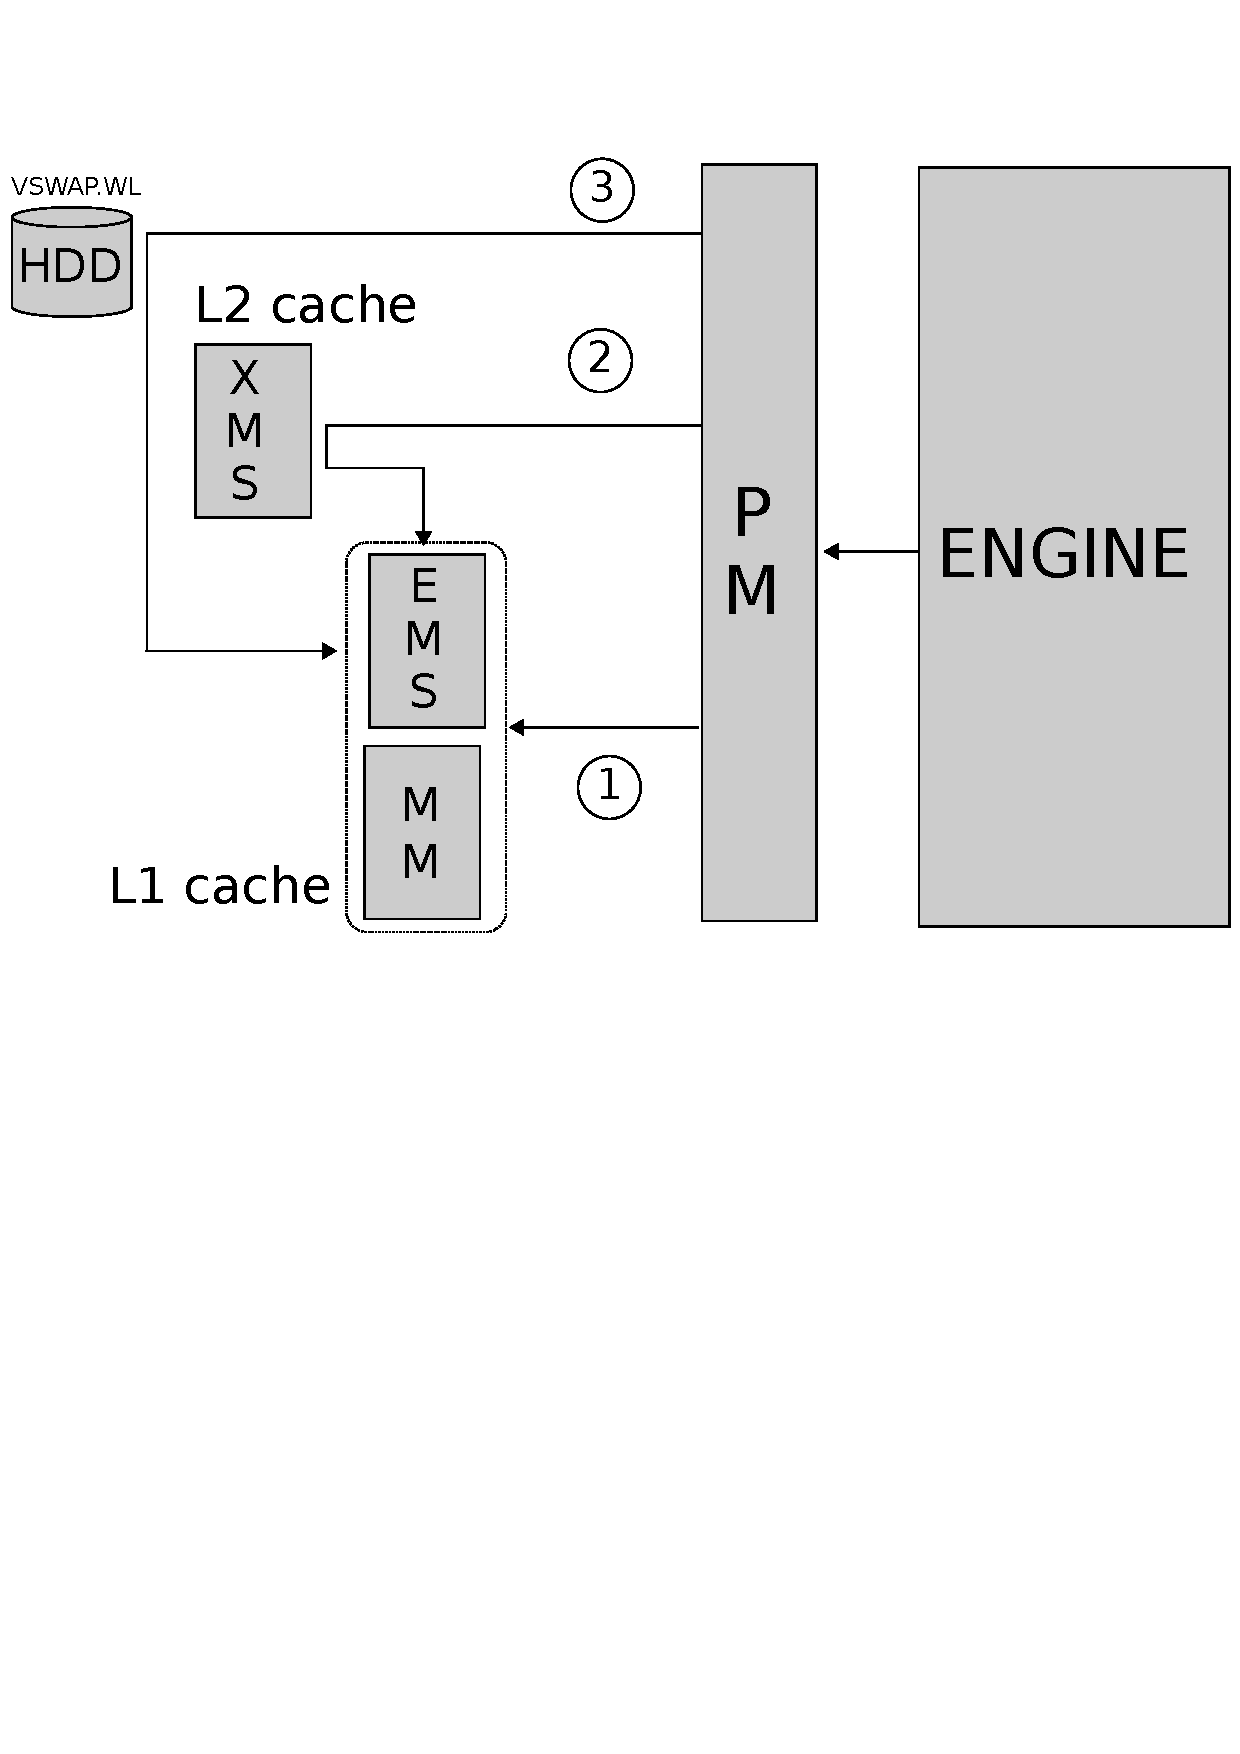
\includegraphics[width=\textwidth]{imgs/drawings/page_manager_architecture.pdf}
 \end{figure}
 \par
 \note{Why is EMS better than XMS? Both rely on banking yet EMS seems to be available without page copying. Something does not add up here. I must have misunderstood the code.}
In order to minimize the cost of page miss, the engine preload the page cache before a level start. This is known at the "Get Psyched" screen:
 \par
\begin{figure}[H]
\centering
 \fullimage{get_psyched.png}
 \caption{The "thermometer" showing the Page Manager precaching process.}
 \end{figure}
 \par
The precaching mechanism is not particularly clever: It loads as many page from the swap file as possible. It doesn't try to look at what is actually used in the level but instead load assets in the order they are stored in \cw{VSWAP} file on the HDD. On a machine with low memory (less than 1MB), the eviction policy (LRU) stabilizes the cache after a few minutes in a level.\\
\par
This design has a small annoying flaw. On a low memory machine a cache miss will occur at the worse possible moment when the player opens the last door of a level and is about to find himself confronted to the heavy powered final boss. An enemy that has never been seen before and therefore not in the cache of the Page Manager. This incurs the worse case of cache miss. One that will requires a long access to the hard-drive, a lag often resulting in an undeserved and humiliating death.\\
\par
The size of the swap file varies depending on the version of the game you play: \cw{VSWAP.WL1} (shareware) is 742KiB while \cw{VSWAP.WL6} (full version) is 1,500KB. In both case a machine with 2MiB of RAM on top of the factory issued 1MiB is enough to have all assets loaded during pre-caching.\\
\par
\bu{Trashing:} When the system has to evict pages but ends up reloading the same resource during the same frame, it is "trashing". The HDD is put to heavy contribution and the framerate drops. Trashing can happen if too many different resources are visible on the screen. In order to help designers balance their creativity with the needs for a decent framerate, the engine detects trashing and flashes the screen border red when it runs in dev-mode.\\
\par
\bu{Sounds are special:} Because the sound cards are fed via a system of interrupt, the sound manager cannot recover from a page miss. Therefore all sound resources are loaded first (they are located at the start of \cw{SWAP.WL1}) and they are only loaded in Conventional memory.











\subsection{Video Manager (VL \& VH)}
The video manager features two parts:
\begin{itemize}
\item A low level dedicated to hardward VGA register manipulation.
\item A high level dedicated to 2D menu drawings.
\end{itemize}
\par






\subsection{Cache Manager (CA)}
A small manager performing a lot since it loads and decompresses map, graphic and music stored on the filesystem and make them available in RAM. Assets of each kind are stored in two files. A header file contains the offset to allow translation from asset ID to byte offset in the data file.\\
 \par
\begin{figure}[H]
\centering
 \includegraphics[width=\textwidth]{imgs/drawings/cache_manager_architecture.pdf}
 \end{figure}
 \par
\bu{Note:} All resources are compressed. In the case of maps and audio the compression is hard-coded in the engine. However for pictures, a third file (\cw{DICT}) contains the compression dictionary to decompress each asset. The Cache Manager handles decompression transparently.\\
\par
\bu{Trivia :} Is it a typo in filename \cw{AUDIOHEA.WL} ? Correct spelling would be \cw{AUDIOHEAD.WL}. Where is the \cw{D}? This is in fact a limitation of the operating system. DOS only allows 8.3 filename (at most eight characters followed by at dot and at most three character for the extension).








\subsection{User Manager (US)}
\begin{minipage}{0.7\textwidth}
Largely based on Catacomb 3D code and written by Jason Blochowiak. The copy/past is very visible since 90\% of the functions declared in the header (ID\_US.H) are not actually implemented in \cw{ID\_US.C}. 
It is a poorly named manager since it takes care mostly of graphic layout. When a \cw{WL\_*} high level routines needs to draw a string, it is passed to \cw{US\_Print} which does all measurement (e.g: Draw string centered)
and then passes these information to the Video Manager (\cw{VW\_DrawPropString}) which takes care of rendition.
\end{minipage}
\begin{minipage}{0.3\textwidth}
\begin{flushright}
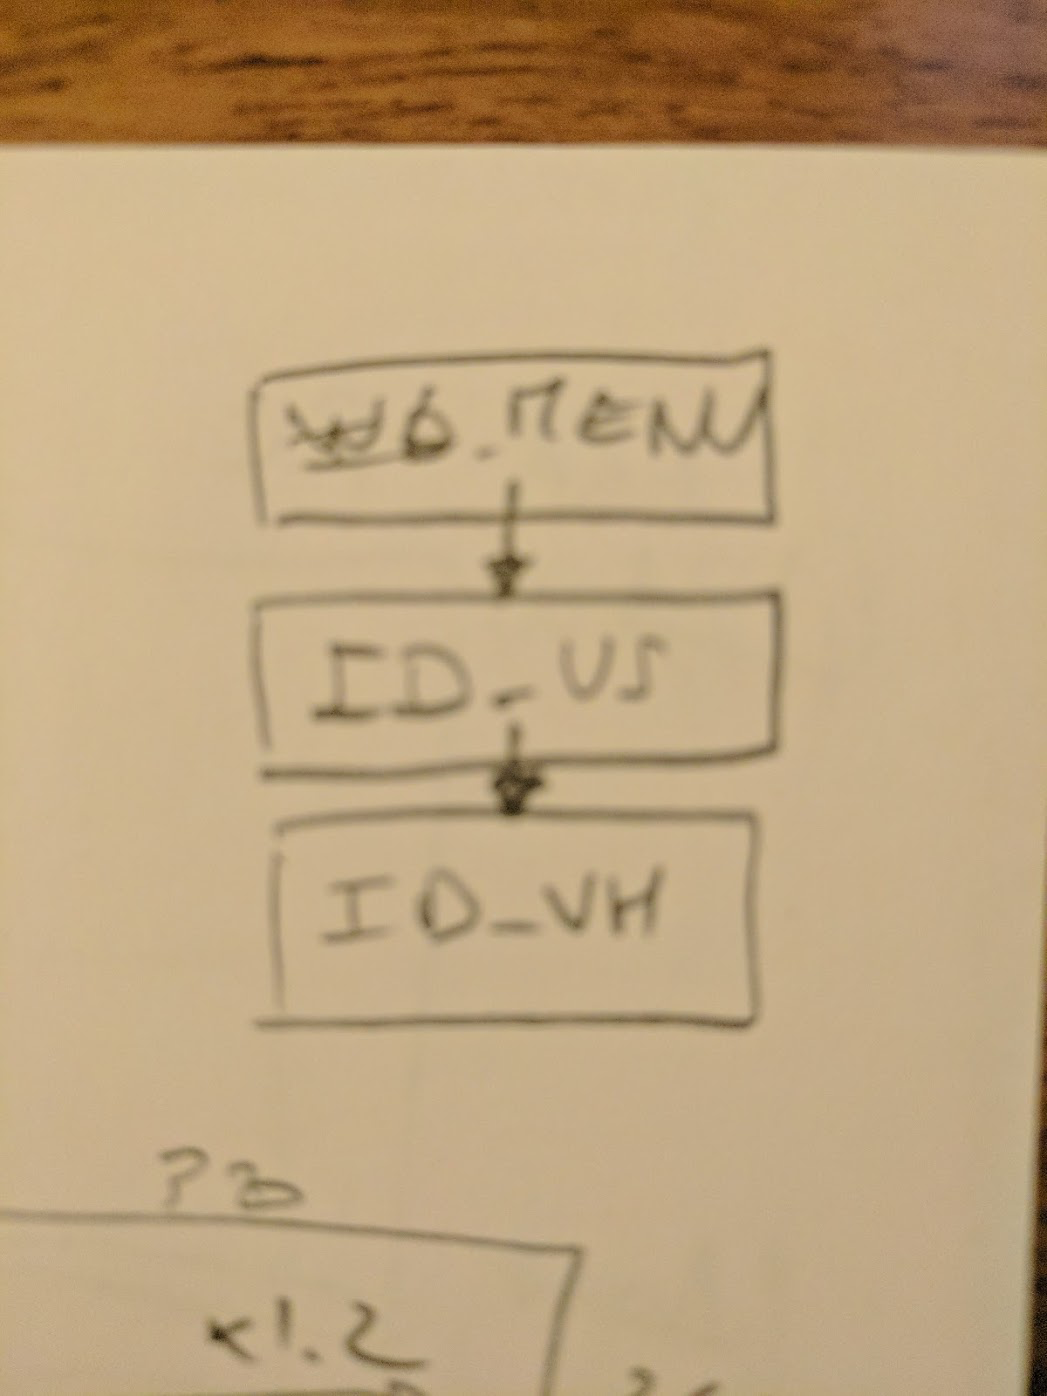
\includegraphics[width=0.8\textwidth]{imgs/drawings/US_explained.pdf}
\end{flushright}
\end{minipage}
\noindent
\\












\subsection{Sound Manager (SD)}
The Sound Manager abstracts interaction with all four sound systems supported: PC Speaker, AdLib, Sound Blaster and SoundSource. It is a beast of his own since it doesn't run inside the engine. Instead it called via IRQ at a much higher frequency than the engine (the engine runs at a maximum 70Hz, the sound manager ranges from 150Hz to 7000Hz). Being IRQ driven, it must run very fast. Therefore not only it is written in assembly, its assets are also privileged when it comes to memory allocation. All of them are loaded in Conventional Memory to avoid a cache miss in the Page Manager.\\
 \par
\begin{figure}[H]
\centering
 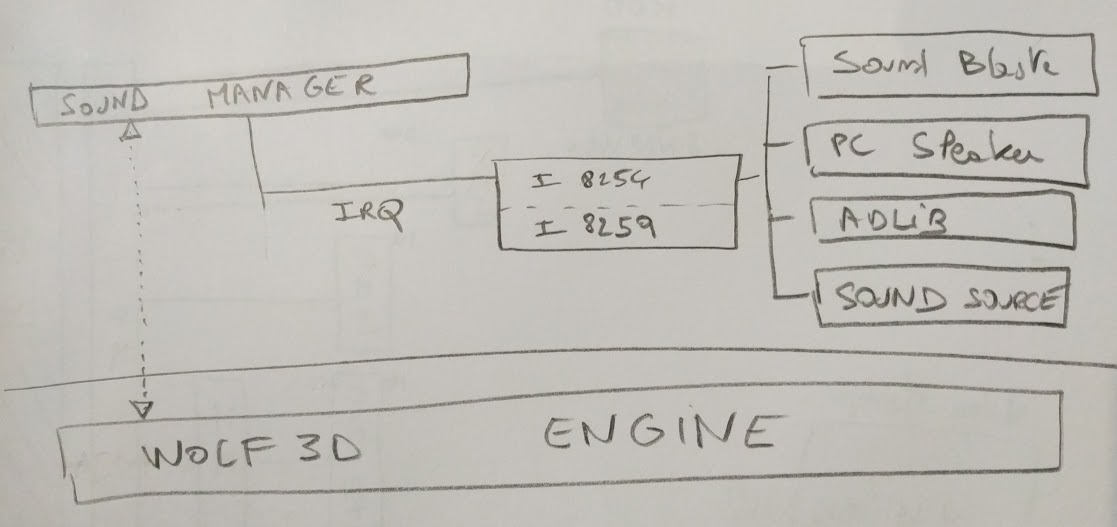
\includegraphics[width=\textwidth]{imgs/drawings/sound_manager_architecture.pdf}
 \end{figure}
 \par
The sound manager is described extensively in the "Sound and Music" section.

















\subsection{Input Manager (IN)}
Abstract interactions with joystick, keyboard and mouse. Features a lot of boring boilerplate code to deal with PS/2, Serial and DA-15 ports. Each using their own I/O addresses.
















\section{Startup}
As the game engine starts, it deals with difficulties showed in the hardware section. This is where things become really interesting.





\subsection{Signon}
The first (mild) issue to deal with is the heterogeneous ecosystem of PCs on the market. With different drivers loaded and different sound cards, the engine has to figure out how much RAM is installed and if it will be able to run. If not it has to let the user know what is the problem. That was important since id Software was a small team and they did not have CSR around to pickup the phone and help unhappy customer to troubleshot their issue.\\
\par
That is what the "signon" screen is for: Self diagnostic. 
\par
\begin{figure}[H]
\centering
\fullimage{signon.png}
\end{figure}
\par
Besides showing recognized devices such as mouse, joystick and sound cards, the most important metric here is labeled "MAIN". Due to the architecture described in the first chapter, a DOS program has only 640KiB of RAM available. Each driver loaded by the user takes away from these 640KB. If too much is used to the point where DOS cannot load the executable in RAM, user will see the following error message.\\
\par 
\begin{minipage}{\textwidth}
\lstinputlisting[language=C]{code/OutOfMemory.txt}
\end{minipage}
\par
The signon screen shows that Wolf3D needs at least 320KiB of Conventional RAM. John Romero wrote a note a release note to help people understand what was going on and avoid angry calls. You can read it in the annex under "The 640KB Barrier".\\
\par 
At the time signon is displayed, the only manager loader is the Memory Manager. There is not even a filesystem for the engine to access yet. That is why the palette and the signon screen are compiled within Wolf3D executable. This is done so they are loaded to RAM by the operating system (DOS) loader. All the engine does is load the palette into the VGA, copy the signon bitmap from RAM to VRAM and fill the blocks with green or yellow based on what was detected.\\
\par
\begin{minipage}{\textwidth}
\lstinputlisting[language=C]{code/signonscreen.c}
\end{minipage}
After that screen, the \cw{introscn} variable (using 320x200 bytes = 64KB) is unloaded from RAM to make more room runtime.\\
\par




















\subsection{Solving the VGA problem}
The Hardware chapter describing the video system left us with an unsolved problem: All of the VGA modes lack double buffering capability.\\
\par
 The most appealing mode (13h) offers a single framebuffer at a resolution of 320x200 non-square pixels with 256 indexed colors. The Chain-4 chipset in the VGA circuitry automatically maps the RAM starting at \cw{A0000h} to the four VRAM banks. 
 \par
 \begin{figure}[H]
\centering
      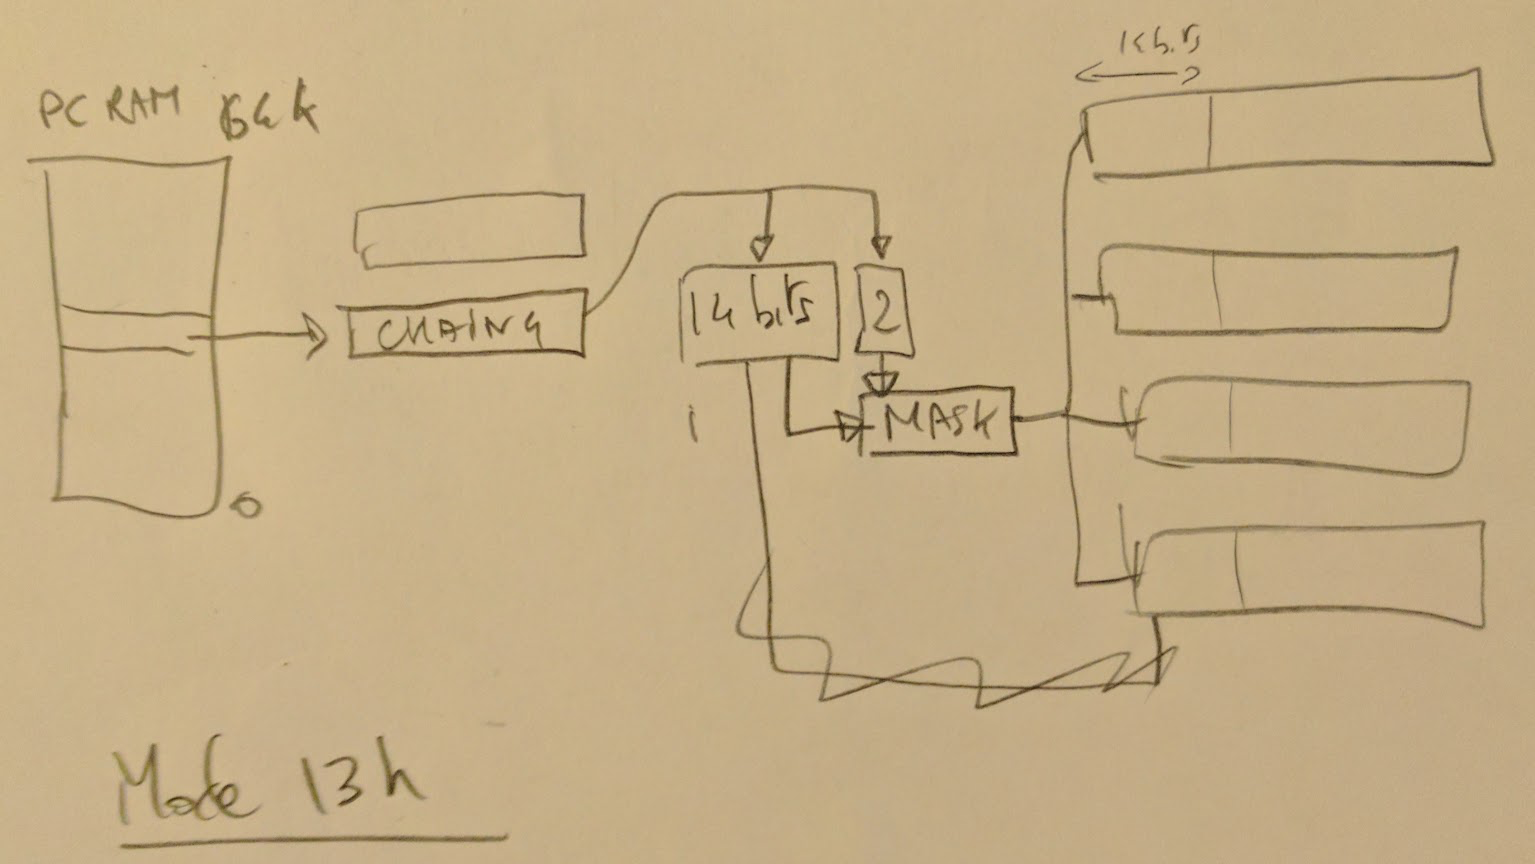
\includegraphics[width=\textwidth]{imgs/drawings/mode_13h.pdf}
\end{figure}

This mapping system is also called "chaining". Because 2 bits out of the address are used to route a write/read operation to a bank, only 14 bits are used for the actual offset in the bank. Since 14 bits can only address 16384 values this system results in 75\% of the VRAM unusable.\\

\begin{figure}[H]
\centering
 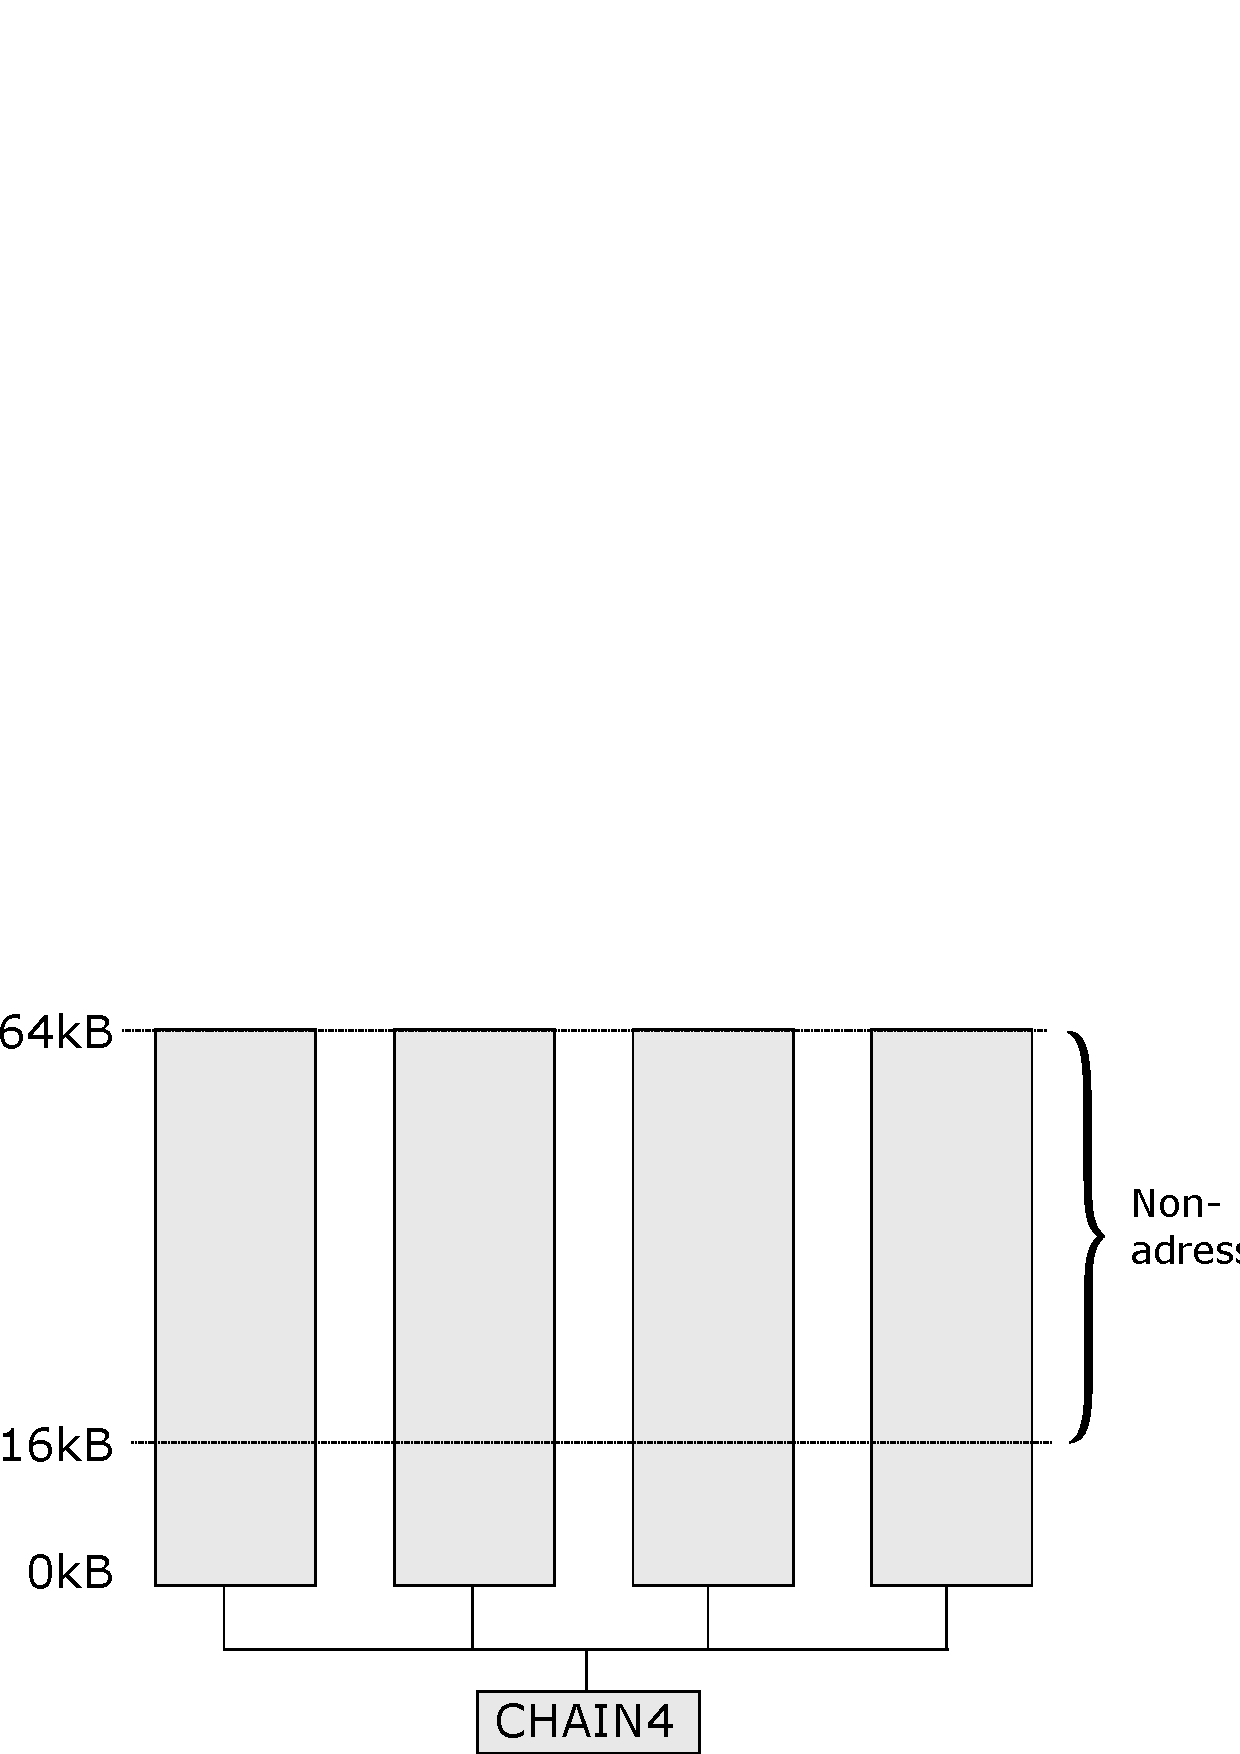
\includegraphics[width=\textwidth]{imgs/drawings/vga_layout/wasted_vga_ram.pdf}
 \end{figure}

 \par
 The waste is really the fault of the Chain-4 chip. Nobody knows who discovered it first but it turns out it is possible to disable it. The technique was popularized by Michael Abrash in Dr. Dobb's Journal of July 1991. In his article he described was he coined the Mode-X. An undocumented sequence of operations disabling Chain-4 allowing a resolution of 320x240, square pixels (since the ration is 4:3) and full access to the 256K of RAM.\\
 \par
 Wolfenstein 3D does things slightly differently. It disables chain-4 but keeps the resolution in 320x200. This mode is known as Mode-Y. \\
 \par
 \bu{Note :} Why not use Mode-X since it gives square pixels ? Despite its advantage for artists, a screen using Mode-Y is 320x200 = 64000 pixels which represent 17\% less pixels compared to Mode-X with 320x240 = 76800 pixels. The engine already struggled to reach an acceptable framerate, Mode-X was simply too many pixels to draw each frames.\\
 \par
\note{Ask John Carmack and John Romero why they went for Mode-Y instead of Mode-X.}
 \par
  \begin{minipage}{\textwidth}
\lstinputlisting[language=C]{code/init_vga.c}
\end{minipage}
 \par

The magic happens in function \cw{VL\_DePlaneVGA} where VGA registers are manipulated to tweak what the BIOS had setup in Mode 13h. \\

 \par
 \begin{minipage}{\textwidth}
\lstinputlisting[language=C]{code/unchaining.c}
\end{minipage}
\note{What is long mode? What is byte mode?}
 \par
 The VGA registers of the Sequence Controller and CRT Controller are setup to divide the VRAM in four parts.
 \begin{itemize}\label{SetupPages}
 \item 64K for Framebuffer 0
 \item 64K for Framebuffer 1
 \item 64K for Framebuffer 2
 \item 64K for Graphic assets
\end{itemize}
\par
\begin{figure}[H]
\centering
 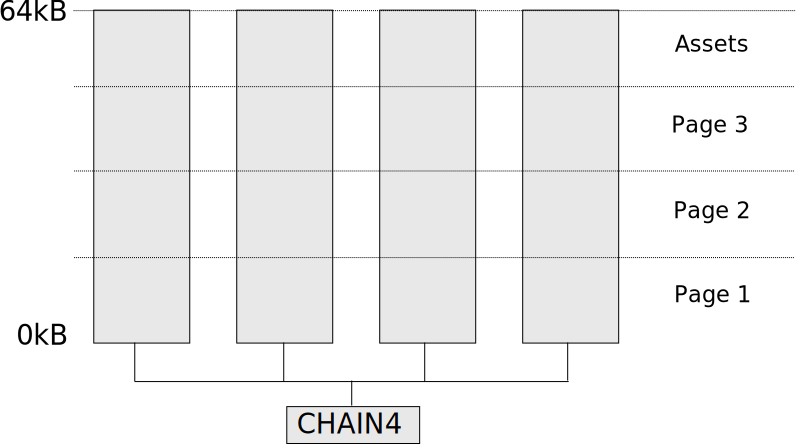
\includegraphics[width=\textwidth]{imgs/drawings/vga_layout/vga_ram_architecture.pdf}
 \end{figure}
\par
But the engine is not done yet. Tweaking Mode 13h into Mode-Y solves one big problem but introduces two smaller ones. One is about speed and the other is about correctness.\\
\par
Let's look at speed first. With chain-4 out of the picture a developer is now in charge of selecting the bank to write to. This can easily be done with a simple function.\\
\par
 \par
 \begin{minipage}{\textwidth}
\lstinputlisting[language=C]{code/select_plan.c}
\end{minipage}
 \par

Now the code sample from the hardware chapter to clear the screen only adds a modulo.\\
\par
\par
\begin{minipage}{\textwidth}
\lstinputlisting[language=C]{code/cleanScreenNaive.c}
\end{minipage}
\par
The code looks innocuous but as simple as it is, it cannot run at more than 5 frames per second. The problem is that we replaced something done in hardware with something done in software. The \cw{outp} instructions are simply too slow.\\
\par
The solution is to change how we draw to the screen. Instead of going top to bottom and left to right, we need to go left to right and top to bottom which minimizes the number of bank switch.\\
\par
\begin{minipage}{\textwidth}
\lstinputlisting[language=C]{code/cleanScreenClever.c}
\end{minipage}

\par
This code can run without issues at 70 frames per second since just 200 slow \cw{out} instructions are used.\\
\par
This speed consideration has a fundamental impact on the engine: To draw anything fast with the VGA, it has to be drawn \underline{vertically}. Everything in the engine is drawn this way: Walls, Sprites, Menu. Everything, absolutely \underline{everything is drawn vertically}. The ramifications of this hardware constraint are felt all the way down to how assets are stored in RAM (rotated 90 degrees) and woven to match the VGA banks layout (this is described in details in the "Rendering sprites" section).\\

\par
The second issue introduced by Mode-Y is about correctness. With three pages available, the engine draws in page 1, then page 2, then page 3 and then goes back to page 1 (notice there are three buffers but this is not triple-buffering). This solves tearing and allows the engine to never stops drawing. It just instructs the CRT Controller that it should scan a framebuffer in VRAM at a new offset after the next vsync.\\
\par
The CRT Controller start scan offset is a 16 bits value which is updated with a little bit of assembly. First the high byte and then the low byte. The code would look as follow.\\
\par
\begin{minipage}{\textwidth}
\lstinputlisting[language={[x86masm]Assembler}]{code/pageflip.c}
\end{minipage}
This code looks like it would work. But there is a major flaw with it. If you were to run it, every once in a while the expected screen.\\
\par
 \begin{figure}[H]
\centering
 \fullimage{full_screen.png}
 \end{figure}
Would instead appear distorted:\\
\par
 \begin{figure}[H]
\centering
 \fullimage{crtc_scanstart_problem.png}
 \end{figure}
\par
This glitch shows part of one page and a part of an other page. It also shows a misalignment. The problem has to do with atomicity. The CRTC starting address is a 16-bits value but the \cw{out} instruction can only write 8-bits at a time. If the pages are setup one after an other like this.
\par
\begin{figure}[H]
 \centering
 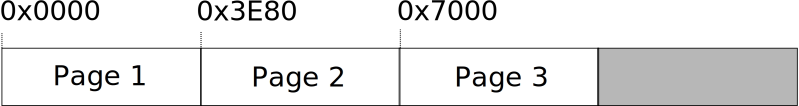
\includegraphics[width=\textwidth]{imgs/drawings/triple_pages_trick.pdf}
\end{figure}
\par
In VRAM, Page 0 is at 0x0000, page 1 at 0x3E80 and page 2 at 0x7000. Instructing the CRTC to use page 1 instead of page 0 requires updating the high byte 0x00 to 0x3E and the low byte 0x00 to 0x80. Since updates are not atomic, given a poor timing the CRTC could pickup a value of 0x3E00 instead of 0x3E80:\\
\par
\par
\begin{minipage}{\textwidth}
\lstinputlisting[language={[x86masm]Assembler}]{code/pageflip_error.c}
\end{minipage}
\par
How do you update atomically a 2 bytes value with 1 byte operation? Take a look at how Wolfenstein setup its pages:\\
\par
\begin{minipage}{\textwidth}
\begin{flushright}
\lstinputlisting[language=C]{code/vga_setup_pages.c}
\end{flushright}
\end{minipage}
\par
Notice how it uses a value of 208 for the height of a framebuffer? That doesn't make sense at first sight since the screen is 200 pixels tall. I thought it was a typo (after all \cw{0} and \cw{8} are visually close) but this was done on purpose. The trick achieved here is to use a little bit of padding after each page so the addresses only differ by their high byte value.


\par
\begin{figure}[H]
 \centering
 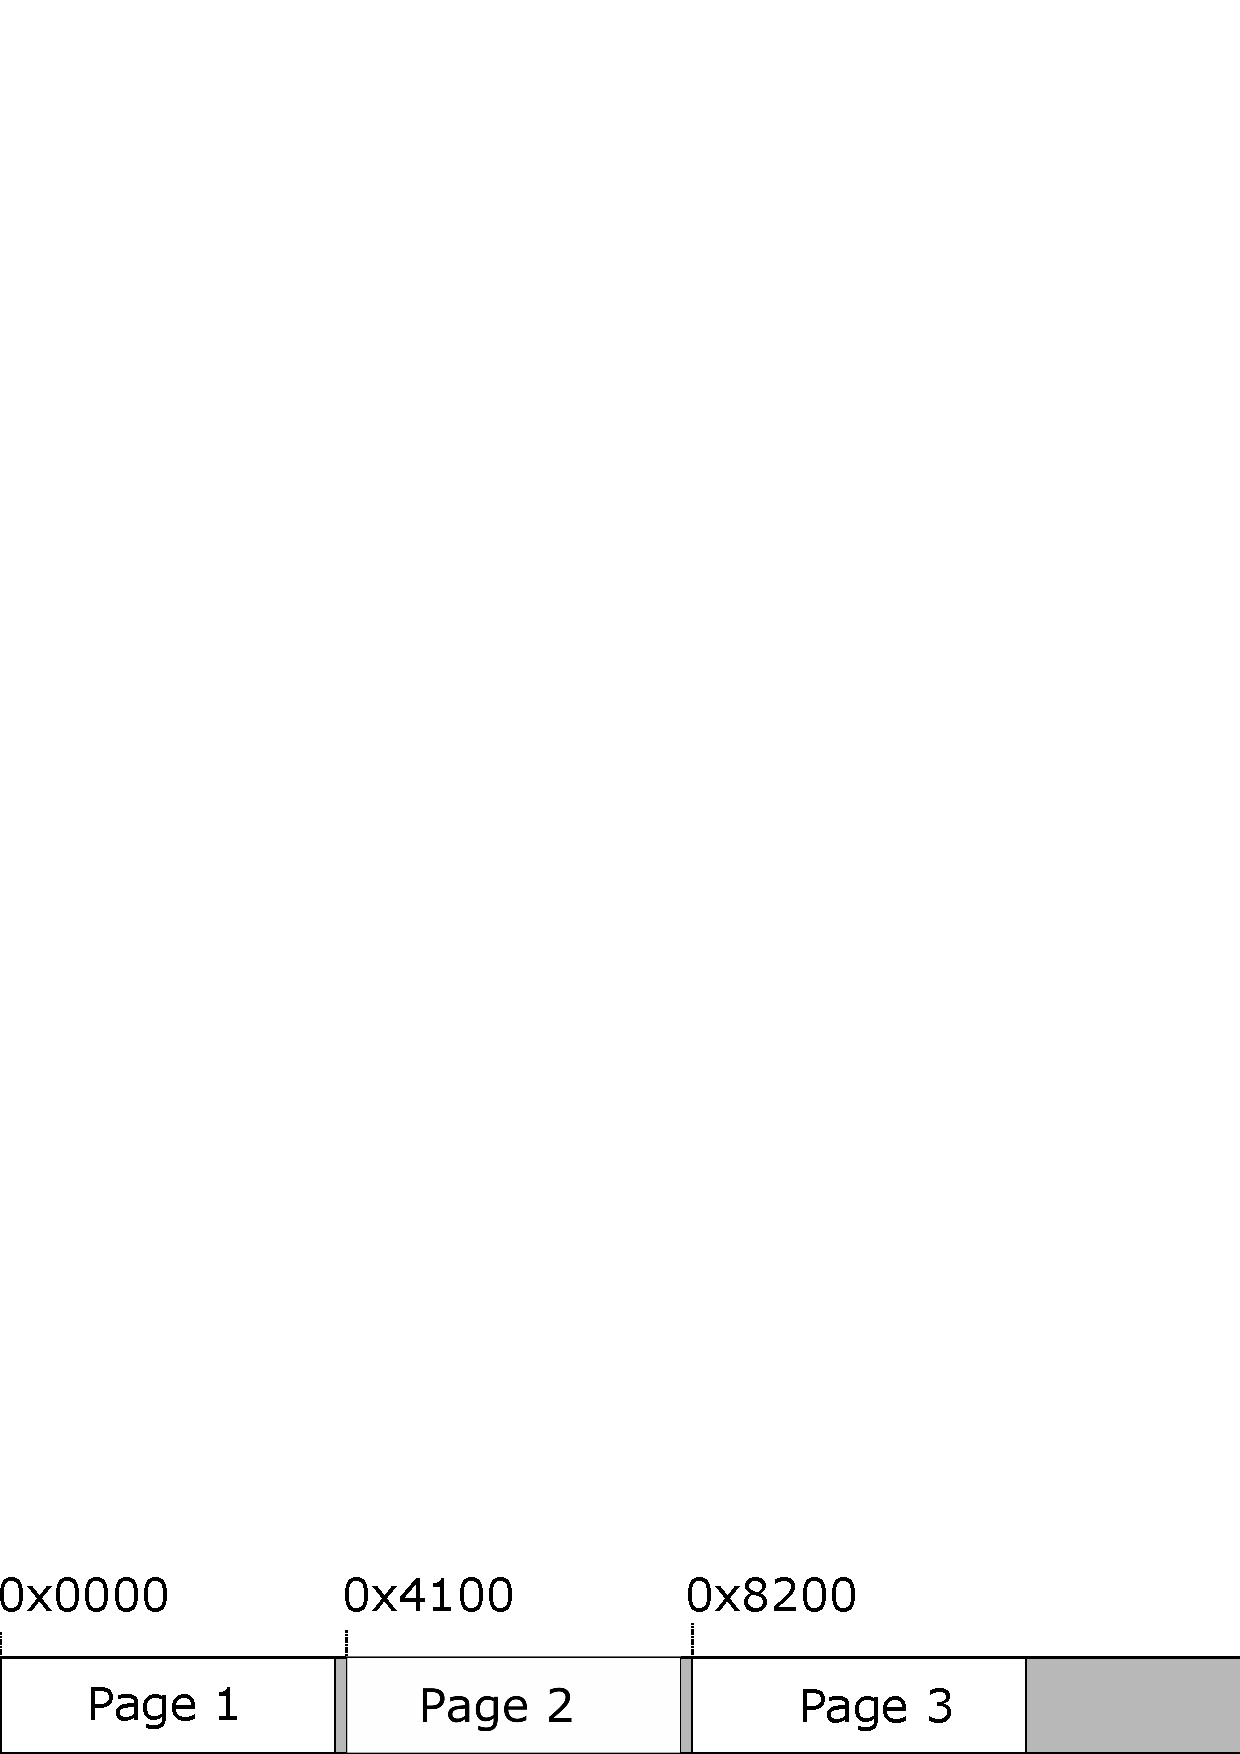
\includegraphics[width=\textwidth]{imgs/drawings/triple_pages_trick_padding.pdf}
\end{figure}
\par



\par
Now page 0 is at 0x0000, page 1 at 0x4100 and page 2 at 0x8200. Moving from any page to an other only requires updating only the high 8 bits, which makes flipping buffer an atomic operation.\\












\subsection{Profound Carnage}
After the signon screen comes a second one, the "rating" screen. There were no official rating for video games in 1991 since the ESRB\footnote{Entertainment Software Rating Board, the organization in charge of assigning age and content ratings.} would not be established until 1994 in response to criticism of controversial video games featuring excessively violent (a.k.a Doom) or sexual content. But the team came up with their own self-proclaimed PC-13: The now legendary "Profound Carnage-13".\\
\begin{figure}[H]
\centering
\fullimage{pg13.png}
\end{figure}







\end{document}
